% Generator: hand-authored TikZ schematic traced from the fixed source; cylinder proportions are illustrative.
% Source ID: src-120ea104f8cb373f5731039fa9d36469df457869849f27420831962ef1ad2306
% PDF SHA-256: d0081500bd56d03199ddcf232fe8e870f2ecd7e9c41ba849417af9af79fbb702
% PDF page 1; printed page 124; question 13.
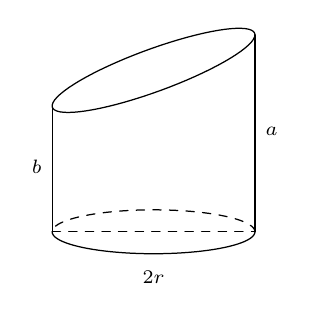
\begin{tikzpicture}[
  x=0.92cm,y=0.82cm,line width=0.45pt,line cap=round,
  every node/.style={font=\scriptsize,inner sep=1.5pt}
]
  % Lower base: dashed rear arc and diameter, solid front arc.
  \draw[dashed,domain=0:180,samples=48,variable=\t]
    plot ({1.4*cos(\t)},{0.34*sin(\t)});
  \draw[domain=180:360,samples=48,variable=\t]
    plot ({1.4*cos(\t)},{0.34*sin(\t)});
  \draw[dashed] (-1.4,0)--(1.4,0);

  % Oblique cut ellipse: the right generator is longer than the left one.
  \draw[domain=0:360,samples=72,variable=\t]
    plot ({1.4*cos(\t)},{2.5+0.55*cos(\t)+0.35*sin(\t)});
  \draw (-1.4,0)--(-1.4,1.95) (1.4,0)--(1.4,3.05);

  \node[left] at (-1.48,1.0) {$b$};
  \node[right] at (1.48,1.55) {$a$};
  \node[below] at (0,-0.54) {$2r$};
\end{tikzpicture}
